After developing and analyzing the different \acs{IoT} system components, it is time to evaluate its overall performance in a real-world scenario. In this chapter, the results of the hospital trial are presented and discussed. 

\section{Hospital Pilot}

For the hospital trial, the proposed \acs{IoT} system was deployed in an clinical facility within Centro Hospitalar e Universitário de Coimbra (CHUC). The trial lasted 3 days, during which 2 volunteers performed 8 hour. 


\begin{figure}[H]
    \centering
    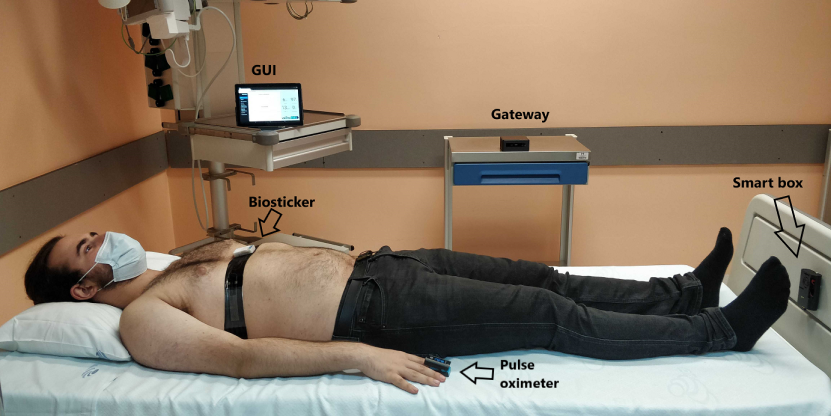
\includegraphics[width=\linewidth]{images/hospital-trial.png}
    \caption[Conceptual illustration of the system components within a medical facility.]{Conceptual illustration of the system components within a medical facility.}
    \label{fig:hospital-trial}
\end{figure}
\dots

To evaluate the performance of the proposed system, 

\begin{itemize}
    \item \acs{MQTT} Communication Latency:
    \item Average \acs{MQTT} Bandwidth over time: 
    \item \acs{FHIR} Communication Latency:
    \item Average \acs{FHIR} Bandwidth over time: 
    \item Average total CPU and RAM usage over time:
\end{itemize}



\section{Results}
\dots

\section{Summary}
In this chapter, the performance of the proposed system during the hospital trial was tested and discussed. 
In the next, and final chapter, an overview of the work achieved is presented in light of the proposed contributions, concluding with some final remarks.